% Journal of Molecular Graphics and Modelling — working submission; not submission-cleared.
% This is a separate derivative of the RSC Advances manuscript.
\documentclass[final,3p,times,twocolumn]{elsarticle}
\usepackage[english]{babel}
\usepackage[T1]{fontenc}
\usepackage{amsmath,amssymb}
\usepackage{graphicx,booktabs,multirow,array,float}
\usepackage{pgf,tcolorbox,enumitem}
\usepackage[detect-all=true,group-minimum-digits=4]{siunitx}
\sisetup{range-phrase=~to~,group-digits=integer,retain-explicit-plus=true}
\usepackage{hyperref}
\usepackage{xr-hyper}
\usepackage{cleveref}
\externaldocument[SI-]{SI_JMGM}
% Working notation shared by the main manuscript and supporting information.
\newcommand{\modelA}{\textsc{Model~A}}
\newcommand{\modelB}{\textsc{Model~B}}
\newcommand{\modelC}{\textsc{Model~C}}
\newcommand{\modelD}{\textsc{Model~D}}
\newcommand{\deltaest}{$\Delta E_\text{ST}$}

\journal{Journal of Molecular Graphics and Modelling}

\begin{document}
\begin{frontmatter}
% Title chosen by author for F3-b re-scope (2026-10-06).
\title{Publication-Level Holdout Separates Fingerprint and Excited-State Descriptor Models of Measured TADF Gaps}
\author[aff1]{Jean-Pierre Tchapet Njafa\corref{cor1}}
\ead{jean-pierre.tchapet@facsciences-uy1.cm}
\author[aff2]{Steve Cabrel Teguia Kouam}
\author[aff1]{Patrick Sorrel Mvoto Kongo}
\author[aff3]{Panebei Samafou}
\author[aff1]{Serge Guy Nana Engo}
\cortext[cor1]{Corresponding author. ORCID: 0000-0002-1936-8353.}
\affiliation[aff1]{organization={Department of Physics, Faculty of Science, University of Yaound\'{e}~1},city={Yaound\'{e}},postcode={812},country={Cameroon}}
\affiliation[aff2]{organization={Department of Physics, Faculty of Science, University of Douala},city={Douala},postcode={24157},country={Cameroon}}
\affiliation[aff3]{organization={Department of Medical Imaging and Radiation Sciences, Faculty of Medicine and Health Sciences, Universit\'{e} de Sherbrooke},addressline={3001, 12th Avenue Nord},city={Sherbrooke},state={QC},postcode={J1H 5N4},country={Canada}}
\begin{abstract}
% JMGM F3-b abstract (2026-10-06; L4 round, trimmed to <=240 words); numbers trace to ledger A-006, A-016--A-020.
Do semi-empirical natural-transition-orbital (NTO) descriptors keep rank
information on measured singlet--triplet gaps \deltaest of thermally
activated delayed fluorescence (TADF) emitters that structural fingerprints
lose when molecules come from publications absent from training? In this
corpus they do. On \num{231} donor--acceptor emitters (\num{173} publications)
from the Huang--Cole TADF database, random forests on GFN2-xTB/sTDA NTO
descriptors order emitters across held-out publications with median
Spearman $\rho = 0.34$, against $0.17$ for Morgan fingerprints. Within a
held-out paper, neither orders molecules.
%
Neither has lower error: scaffold-cross-validated mean absolute errors are
\qty{0.091}{\electronvolt} (Morgan) and \qty{0.096}{\electronvolt} (NTO), paired
difference \qty{95}{\percent} CI \numrange{-0.017}{0.009}\,\unit{\electronvolt},
both \numrange{10}{15}\,\unit{\percent} below a mean-value predictor.
%
NTO minus Morgan $\Delta\rho$ is $0.16$ under source-paper holdout (central \qty{95}{\percent} of
\numrange{0.07}{0.25} over \num{50} fold assignments); NTO ranks higher in
\num{19} of \num{20} paper partitions, against \num{11} and \num{13} of \num{20}
for matched scaffold and molecule partitions. NTO $\rho$ barely moves across
units, whereas Morgan $\rho$ falls from $0.31$ to $0.17$ and RDKit 2D
descriptors from $0.30$ to $0.21$. The contribution is this matched three-unit
holdout comparison: fingerprint and RDKit ranking depends on same-publication
molecules in training, NTO ranking does not. This is an association: siblings
share structure and measurement protocol.
%
Inter-report scatter caps $R^2$ near \numrange{0.80}{0.86}, above the observed
$0.26$. No laboratory transfer was tested. Here, random or scaffold splits
overstated fingerprint ranking skill; source-publication holdout should
accompany them.

\end{abstract}
\begin{keyword}
Thermally activated delayed fluorescence \sep singlet--triplet gap \sep molecular modelling \sep excited-state descriptors \sep machine learning \sep cross-validation
\end{keyword}
\end{frontmatter}

% ============================================================
% JMGM Introduction — F3-b re-scope (2026-10-06)
% Central question: do semi-empirical NTO descriptors retain rank information on
% measured TADF gaps that fingerprints lose on publications absent from training?
% Numbers trace to ledger A-006, A-007, A-016--A-020 and the Results section.
% ============================================================

\section{Introduction}\label{sec:introduction}

\subsection{Predicting the singlet--triplet gap of TADF emitters}

Thermally activated delayed fluorescence (TADF) emitters---organic donor--acceptor
molecules that harvest both singlet and triplet excitons for near-unity internal
quantum efficiency~\cite{Uoyama2012}---are the heavy-metal-free route to tunable,
efficient light sources for displays and for human-centric and horticultural
lighting~\cite{Yokoyama_2018, Bugbee2016}. An efficient emitter has to meet several
requirements at once: a small singlet--triplet gap
($\Delta E_\text{ST} < \qty{0.2}{\electronvolt}$), fast reverse intersystem crossing
($k_\text{RISC} > \qty{1e6}{\per\second}$), and emission matched to the target band.
This paper addresses only the first. The rate and device-efficiency requirements need
spin--orbit-coupling and device-level calculations beyond the cheap structural data
used here, and we make no quantitative claim about them (\cref{subsec:limitations}).

\subsection{Machine learning on computed and measured gaps}

Designing such emitters means searching a large space of donor--acceptor
combinations for a small $\Delta E_\text{ST}$. The direct route---time-dependent
DFT on excited states---scales steeply with system size~\cite{Curtarolo2013},
so exhaustive screening of more than a few hundred candidates is impractical.
Machine learning offers a cheaper surrogate~\cite{Butler2018, Pyzer-Knapp2022},
and several groups have predicted TADF gaps from molecular
descriptors~\cite{Gomez-Bombarelli2016, Barneschi2024}. Those low reported errors
are obtained against \emph{computed} (TD-DFT or higher) reference gaps. Nigam
et al.~\cite{Nigam2024} also worked with computed labels, gaps simulated at the
$\omega$B2PLYP$'$ level, and replaced an early regression model with a good/bad
classifier (\cref{subsec:comparison}); their study does not show how models behave
on measured gaps. The closest prior work on measured gaps is that of He
et al.~\cite{He2026}, who trained machine-learning models on \num{1321}
experimental $\Delta E_\text{ST}$ records with measurement-condition features.
Neither study compares a structural fingerprint with a semi-empirical
excited-state representation under molecule, scaffold and source-publication
holdout, which is the comparison made here.
Experimental molecular-property learning is not, by itself, a new approach:
JMGM studies have combined explainable predictors with experimental
ligand--receptor observations~\cite{Ferri2026TAS2R} and modelled experimental
infrared peaks~\cite{Noreen2026IR}. Our question concerns the representation and
the unit that is held out.

One problem recurs in this literature. Accuracy is often quoted against a single random train--test split, which rewards
interpolation within familiar scaffolds and overstates how a model behaves on new
chemistry. Literature-mined corpora sharpen this problem: one publication usually
reports a series of close analogues measured under one protocol, so a random or
scaffold split leaves same-paper siblings of a test molecule in training.

Our earlier work set the stage: Article~1~\cite{Tchapet2024_xTB} benchmarked in JCIM
GFN2-xTB/sTDA against \num{747} experimental molecules
(MAE = \qty{0.162}{\electronvolt}), xTB geometry relaxations, and scaffold
cross-validation, and Article~2~\cite{Tchapet2024_DataDriven}
extracted structure--property design rules from that set. Here we ask: do
semi-empirical natural-transition-orbital (NTO) descriptors retain rank information
on measured TADF singlet--triplet gaps that structural fingerprints lose when
molecules come from publications absent from training? The measured gaps come from
the ChemDataExtractor-generated TADF database of Huang and Cole~\cite{HuangCole2024};
after matching to our descriptor set they cover \num{231} donor--acceptor emitters
from \num{173} publications.

\subsection{Our contributions}

We compare error and rank ordering under three holdout units rather than claim a
new high-accuracy predictor. The answer to the question is yes, within this
corpus: under source-paper holdout the NTO model orders emitters across
publications absent from training with median Spearman $\rho = 0.34$, against
$0.17$ for Morgan fingerprints. Neither representation orders molecules within a
held-out paper, and neither has lower error than the other. The points below
follow the order of the Results.

\paragraph{Fingerprint and NTO models have similar error.}
On \num{231} molecules across \num{212} Bemis--Murcko scaffolds, random forests built
from the 2D structure alone---Morgan fingerprints (MAE = \qty{0.091}{\electronvolt}) and
RDKit descriptors (\qty{0.100}{\electronvolt})---match descriptors derived from a
semi-empirical excited-state calculation (NTO spatial features,
\qty{0.096}{\electronvolt}); the Morgan and NTO models sit only \qtyrange{10}{15}{\percent}
below a mean-value predictor (\qty{0.107}{\electronvolt}). The paired MAE difference is $-\qty{0.0043}{\electronvolt}$ for Morgan minus NTO
(\qty{95}{\percent} CI \qtyrange{-0.0171}{+0.0092}{\electronvolt}). The error
comparison does not move with the holdout unit: under source-paper holdout the
median Morgan-minus-NTO difference is \qty{-0.0004}{\electronvolt}. Unlike a
physics-guided model trained on NTO descriptors against a \emph{computed} reference
gap~\cite{Das2025}, we test the same class of descriptor against the
\emph{measured} gap.

\paragraph{Fingerprint ranking depends on same-publication molecules.}
Over \num{50} random fold assignments, the NTO-minus-Morgan rank difference is
$\Delta\rho = 0.160$ under source-paper holdout (range \numrange{0.07}{0.25}),
against \num{0.073} under scaffold and \num{0.055} under molecule holdout; NTO ranks
higher in \num{19} of \num{20} repeated paper partitions, against \num{11} and
\num{13} of \num{20} for matched scaffold and molecule partitions. The ranges
describe fold-assignment variability, not confidence intervals. NTO $\rho$ stays
between \num{0.337} and \num{0.352} across units; Morgan $\rho$ falls from
\num{0.305} to \num{0.172}. The drop sits on molecules with same-paper siblings:
for them Morgan $\rho$ is \num{0.54} when siblings are in training and \num{0.26}
when the paper is held out, while on the \num{128} molecules from single-molecule
papers it is \num{0.10} under either holdout. NTO is higher on those molecules, but
the seed-averaged NTO-minus-Morgan contrast there ($\Delta\rho = \num{0.16}$,
\qty{95}{\percent} CI \numrange{-0.05}{0.37}) is not resolved. RDKit 2D
descriptors lose rank under paper holdout as Morgan does ($\rho$ \num{0.303} to
\num{0.209}), so among the three sets tested the invariance belongs to the NTO
descriptors. NTO orders emitters across publications absent from training; no
representation orders molecules within a held-out paper. Siblings share close
structure and measurement protocol, and these tests cannot separate the two, so we
report the dependence as an association.

\paragraph{Label scatter leaves room the models do not use.}
Independent experimental reports for the same compound scatter by
\qty{0.072}{\electronvolt} RMS (the largest within-molecule standard deviation is
\qty{0.56}{\electronvolt}). For the \num{102} molecules with several reports, the
median label has an RMS standard error of \qty{0.049}{\electronvolt}; counting the
\num{129} single-report labels at single-report scatter, label noise over all
\num{231} molecules is about \qty{0.072}{\electronvolt} RMS.
Individual discrepancies in reported $\Delta E_\text{ST}$ have been noted for
TADF emitters~\cite{Shuaib2026}; here we quantify inter-report variability
across the \num{231}-molecule corpus drawn from \num{173} papers.
Applying the noise-ceiling framework of Crusius et al.~\cite{Crusius2025} with
per-molecule label noise gives $R^2_\text{max} \approx 0.80$--\num{0.86}
(\cref{subsec:ceilings}), well above the observed $R^2 \approx 0.26$, so label
noise is not the dominant limit and it does not establish a
\qty{0.1}{\electronvolt} MAE floor. Computed references face a separate limit:
B3LYP and CAM-B3LYP gaps differ by up to \qty{0.58}{\electronvolt}. On this corpus
neither a higher-capacity tabular learner (gradient boosting, MLP, SVR) nor the one
frozen pretrained molecular-transformer embedding we tested beats the random forest
(the latter reaches MAE \qtyrange{0.109}{0.113}{\electronvolt}). Low-gap enrichment
on held-out labelled data (\numrange{1.2}{1.4}$\times$ over random) and a filtered
virtual library are reported in the SI; neither supports molecule-level selection,
and we make no device-level performance claims.

This study builds on our earlier work---\textbf{Article~1}~\cite{Tchapet2024_xTB}
(xTB/sTDA validation) and \textbf{Article~2}~\cite{Tchapet2024_DataDriven} (design
rules)---by testing how the holdout unit changes the comparison on measured labels.
The measured labels come from the Huang--Cole TADF database~\cite{HuangCole2024}.
Data, code and the analysis ledger for the three related articles are archived under
Zenodo concept DOI 10.5281/zenodo.17436069 (latest version) and mirrored on GitHub; the
scripts and outputs of the holdout analyses reported here are in that archive and are
also supplied as Supplementary Data (see the Data and code availability statement).

The contribution of this work is a matched comparison of three holdout units
(molecule, scaffold and source publication) on the same \num{231} measured gaps,
which shows that fingerprint and RDKit ranking of measured TADF gaps depends on
same-publication molecules in training while semi-empirical NTO ranking does not.
The error null carries its own information. Because the NTO and fingerprint models
do not differ in error, the sTDA calculation is not
justified by accuracy; its measurable value is ranking across publications. The
\qtyrange{10}{15}{\percent} gain over the mean-value predictor is the margin a new
structure representation has to beat on these labels.

% ============================================================
% JMGM Methods — F3-b re-scope (2026-10-06). Numbers trace to the ledger and
% the scripts in code/.
% ============================================================

\section{Methods}\label{sec:methods}

\subsection{Experimental target and dataset}\label{para:validation_hierarchy}

The prediction target is the \emph{experimental} singlet--triplet gap
$\Delta E_\text{ST}$. We took literature-reported values from the ChemDataExtractor-generated TADF
database of Huang and Cole~\cite{HuangCole2024} and matched them, by compound name, to molecules in
our descriptor set, retaining values in the physical range
\qtyrange{-0.3}{1.5}{\electronvolt}. Where a compound carried multiple independent
reports we used the median and recorded the inter-report spread; a single report sits
\qty{0.072}{\electronvolt} from the median (RMS, weighting each molecule equally; the
report-pooled value is \qty{0.0905}{\electronvolt}). For the \num{102} multi-report
molecules the median carries an RMS standard error of \qty{0.049}{\electronvolt}; with the
\num{129} single-report labels counted at single-report scatter, the label noise over all
\num{231} molecules is about \qty{0.072}{\electronvolt} RMS (\cref{subsec:ceilings}). The final benchmark comprises \num{231} donor--acceptor
molecules spanning \num{212} distinct Bemis--Murcko scaffolds~\cite{Bemis1996}.

Each molecule was assigned one \emph{primary DOI}: the source publication that contributes
the most reports for that molecule (ties are broken by the
code's report-count ordering). This gives \num{173} primary-DOI groups for the \num{231} molecules, of
which \num{128} contain one molecule and \num{45} contain more than one
(\texttt{code/jmgm\_doi\_group\_ranking\_check.py}).

The corpus does not record measurement medium (solvent, host) for individual
values, so the per-molecule median is a consensus over uncontrolled conditions
rather than a single, solvent-specific state. Because environmental electrostatics
and conformational disorder are recognised as primary obstacles to accurate TADF
modelling,\cite{Olivier2017} this consensus is best read as the central tendency of
experimentally accessible $S_1$--$T_1$ gaps; it trades physical specificity for
reduced variance. For the \num{102} molecules with repeat reports, a single random
report deviates from this median by \qty{0.072}{\electronvolt} on
average---comparable to the model error itself
(Table~\ref{SI-tab:solvent}). For those molecules the median is known more precisely,
to \qty{0.049}{\electronvolt} RMS standard error.

The sTDA $S_1$ and $T_1$ energies are excluded from the NTO set because supplying them
reproduces a computed gap exactly: under scaffold cross-validation a linear model given
both energies recovers $E_{S_1}-E_{T_1}$ with $R^2 = 1.000$, and a random forest reaches
$R^2 = 0.59$ on the same features (Section~\ref{SI-sec:leakage}).

\subsection{Cheap electronic-structure inputs and physics-informed descriptors}

Excited-state quantities used to build descriptors were obtained at the
semi-empirical level: GFN2-xTB~\cite{Bannwarth2019} geometries
(\texttt{xtb} version 6.7.1) followed by sTDA~\cite{Grimme2017} for the lowest singlet
and triplet states. From the natural transition orbitals
(NTOs)~\cite{Martin2003} of each excitation we computed spatial overlap
descriptors that encode exchange-integral physics:
\begin{align}
  S_\text{he} &= \int \phi_\text{hole}(\mathbf{r})\,\phi_\text{electron}(\mathbf{r})\,d\mathbf{r}, \label{eq:overlap}\\
  \Delta\lambda_\text{A} &= |\lambda_\text{A}(S_1) - \lambda_\text{A}(T_1)|, \label{eq:delta_lambda}\\
  \text{Char}_\text{diff}^2 &= \Big[\textstyle\sum_i |q_i(S_1) - q_i(T_1)|\Big]^2, \label{eq:char_diff}\\
  \Delta S_\text{he} &= |S_\text{he}(S_1) - S_\text{he}(T_1)|. \label{eq:delta_overlap}
\end{align}
$S_\text{he}$ quantifies hole--electron overlap (related to the exchange
integral), $\Delta\lambda_\text{A}$ acceptor-participation differences,
$\text{Char}_\text{diff}^2$ charge-transfer character changes, and
$\Delta S_\text{he}$ the singlet--triplet overlap difference. The full set of
\num{35} NTO descriptors (the $S_1$/$T_1$ energy scalars excluded) is listed in
the Supporting Information; these descriptors require the sTDA excited-state
calculation, even though they omit the energies themselves.
The ground-state wavefunction for sTDA was generated with \texttt{xtb4stda}, and
excitations were computed with \texttt{stda -xtb -e 10} (sTDA-xTB parametrisation,
\qty{10}{\electronvolt} excitation-energy window; \texttt{-t} for triplets), all in the
gas phase; descriptors use the sTDA rather than the sTD-DFT (\texttt{-rpa}) results.

\subsection{Feature sets and machine-learning models}

We compared three feature representations on the same molecules. Two require no
quantum chemistry, being computed from the 2D structure alone:
(i)~RDKit physicochemical descriptors~\cite{Landrum2016} and (ii)~Morgan
fingerprints (radius~2, \num{2048} bits; RDKit
\texttt{GetMorganFingerprintAsBitVect} with its defaults, i.e.\ no chirality and
no feature invariants). The third, (iii)~the NTO spatial
descriptors above, is derived from the sTDA excited state but excludes the energy
scalars. A reference set that additionally includes the sTDA $S_1$/$T_1$
energies was also evaluated. We used random-forest
regressors~\cite{Breiman2001} (\num{400} trees, scikit-learn~\cite{Pedregosa2011}),
which outperformed support-vector regression, ridge regression and a mean-value
baseline on this task.

\paragraph{Evaluation.}
Error metrics, \cref{tab:feature_comparison}, the baselines of Table~\ref{SI-tab:baselines}, the SHAP analysis and the
label-noise analyses use Bemis--Murcko scaffold \texttt{GroupKFold} ($k=5$); the
source-paper (DOI-grouped) results and the holdout-unit controls below use the
holdout unit stated with each number. Because \qty{92.9}{\percent} of scaffolds are singletons, this split is
numerically close to a random split; we therefore also report five-fold source-paper
(DOI-grouped) out-of-fold predictions. That grouping holds out source publications and any synthetic
series or measurement practices correlated with them, but does not identify a
laboratory or control the protocol (\cref{subsec:benchmark}). The corpus records
no solvent, host or temperature per value, so a paper DOI is only a proxy for
shared conditions, not a measured protocol.
We benchmark against a mean-value predictor, the raw sTDA gap, and a
range-separated TD-DFT reference gap (\cref{subsec:benchmark}), and report
\qty{95}{\percent} confidence intervals from \num{2000} bootstrap resamples of the
out-of-fold predictions.
For the DOI-grouped rank contrast, we also resampled the \num{173} primary DOI
groups as clusters (\num{5000} paired percentile-bootstrap draws, seed \num{54321})
while keeping the original out-of-fold predictions fixed. As a partition
sensitivity check, we refitted both random forests in \num{20} source-paper
\texttt{GroupShuffleSplit} partitions (\qty{20}{\percent} of DOI groups held out;
seed \num{17}) and computed Spearman correlation on each test partition. These
overlapping partitions are descriptive, not independent confirmations or a
confidence interval for new laboratories.

\paragraph{Holdout-unit controls.}
To separate the effect of the holdout unit from the effect of the error-versus-ranking metric,
we compared three units on the same \num{231} molecules: single molecule (random
folds), Bemis--Murcko scaffold (\num{212} groups) and primary source publication
(\num{173} groups). For each unit we drew \num{50} random assignments of groups to
\num{5} folds, fitted both random forests (\num{400} trees) on each assignment and
computed pooled out-of-fold Spearman $\rho$ and MAE for Morgan and NTO features. The
spread over the \num{50} assignments (2.5th--97.5th percentiles) describes
fold-assignment variability; it is not a confidence interval. The \num{20}-partition
\texttt{GroupShuffleSplit} count was repeated for each unit. On a fixed scaffold split we
also resampled scaffold clusters (\num{5000} draws). The same \num{50} assignments were
reused to split the molecules into \num{103} from papers with at least one other molecule
in the corpus (multi-molecule papers) and \num{128} from single-molecule papers, and
to compute (i)~$\rho$ within each subset and (ii)~a sibling-pull statistic, the Spearman
correlation between a molecule's out-of-fold prediction and the leave-self-out mean
label of the other molecules from the same paper (\num{103} molecules). Code:
\texttt{code/a017\_split\_unit\_controls.py} and
\texttt{code/a019\_series\_shortcut\_test.py}; outputs in
\texttt{data/a017\_split\_unit\_controls.json} and
\texttt{data/a019\_series\_shortcut\_test.json}. The same \num{50} molecule- and
paper-holdout assignments were repeated with the \num{217} RDKit 2D descriptors, and
within-paper ranking was measured as the Spearman correlation between paper-centred
labels and paper-centred predictions on the \num{103} multi-paper molecules. For the
\num{128} single-paper molecules, out-of-fold predictions were averaged over the \num{50}
paper-holdout assignments and the NTO-minus-Morgan $\rho$ difference was given a paired
molecule bootstrap interval (\num{5000} draws, seed \num{54321}); code
\texttt{code/a020\_controls.py}, output \texttt{data/a020\_controls.json}. These analyses
(\texttt{a017}--\texttt{a020}) were designed after the fixed-split result
(\texttt{a016}) had been seen; the decision rule of each was fixed before it was run and
is recorded in the script's docstring. Code and full per-split values for
the fixed split are in \texttt{code/jmgm\_doi\_group\_ranking\_check.py} and
\texttt{data/a016\_jmgm\_doi\_group\_ranking.json}.

\paragraph{TD-DFT reference gap.}
For a higher-level reference we computed vertical \deltaest\ for all \num{231}
molecules at wB97X-D4/def2-SVP with RIJCOSX and the Tamm--Dancoff approximation
(ORCA~6~\cite{Neese2020}; \texttt{nroots}~8, triplets included; GFN2-xTB
ground-state geometry). All \num{231}/\num{231} jobs converged
(\qty{76.2}{\hour} elapsed on \num{8} processes, so \num{609} core-hours; median
\qty{16.1}{\minute} per molecule, slowest \qty{2.1}{\hour}). These are measured wall times
from \texttt{results/tddft\_reference\_231.csv}, not a scaling extrapolation. The raw
gap, an in-fold linearly calibrated gap, and the gap as an added descriptor in
the random forest model are evaluated against the mean-value baseline on the same
scaffold and DOI cross-validation folds (\cref{subsec:benchmark};
Table~\ref{SI-tab:tddft_headtohead}).
B3LYP/6-31G(d) and CAM-B3LYP/def2-TZVP calculations on \num{7} emitters (functional
dependence of the computed gap), and CAM-B3LYP/def2-TZVP calculations on \num{14}
emitters (adiabatic gaps and the
$T_1$--$T_2$ manifold) are described in Section~\ref{SI-sec:dft_benchmark}; the
substructure-filtered PubChem library is described in Section~\ref{SI-sec:library}.

\paragraph{Interpretability and reproducibility.}
Feature importance was quantified with exact TreeSHAP~\cite{Lundberg2017} on the
fitted forest. All scripts (\texttt{code/finalize\_model.py},
\texttt{code/rebuild\_structural\_model.py}) regenerate every reported number and
\cref{fig:model_performance}.
Software: scikit-learn~1.8.0 and RDKit~2026.03.2. Every random forest used
\num{400} trees, \texttt{random\_state}~=~0 and otherwise scikit-learn defaults.
The \num{50} fold assignments per holdout unit were drawn with NumPy generator
seeds 0, 1, \ldots, 49 (one seed per assignment,
\texttt{numpy.random.default\_rng(seed)}); the paper-cluster, scaffold-cluster
and molecule bootstraps used seed \num{54321}, and the \num{20}
\texttt{GroupShuffleSplit} partitions used seed \num{17}. Data source, splits,
features, model, hyperparameters, metrics and code location are collected in
Table~\ref{SI-tab:ml_reporting}.

\paragraph{Bootstrap confidence intervals and power analysis.}
Point estimates of the rank correlation are complemented by
\num{5000}-replicate percentile bootstrap confidence intervals on the
out-of-fold predictions (\texttt{code/r2\_ci\_power\_analysis.py}).
For the headline model the Spearman $\rho = 0.36$ ($n = 231$) has a \qty{95}{\percent}~CI of
\numrange{0.24}{0.47} ($p = \num{2.6e-8}$) and the Pearson $r = 0.50$ a \qty{95}{\percent}~CI
of \numrange{0.26}{0.68}; both exclude zero, establishing statistically
significant association despite the wide $R^2$ interval.
A power analysis for the correlation test (Fisher $z$ transform, two-sided,
$\alpha = 0.05$) shows that detecting $\rho = 0.36$ at \qty{80}{\percent} power
requires only $n \approx 60$ (\qty{90}{\percent} power: $n \approx 79$); at
$n = 231$ the achieved power is $\approx 1.0$. This bears on the ranking question only:
it establishes that the $\rho$ estimate is not sample-size-limited, and it says nothing
about the width of the $R^2$ interval, which is a different statistic and is discussed on
its own terms in \cref{subsec:benchmark}. We report Spearman~$\rho$ as the primary metric
for triage utility because triage is a ranking task, not because it is the more favourable
number; the full set of metrics and intervals is collected in
Table~\ref{SI-tab:metrics_ci}.

\subsection{Data and code availability}

Labels: Huang--Cole TADF database~\cite{HuangCole2024}. Data, code and the full
analysis ledger for the three related articles: Zenodo concept DOI 10.5281/zenodo.17436069
(latest version), mirrored on GitHub (Data\_Articles\_TADF). The holdout-analysis scripts
and outputs (A-016 to A-020) are in that archive (	exttt{ML\_reproducibility/code},
	exttt{ML\_reproducibility/data}) and are also enclosed as Supplementary Data
(	exttt{supplementary\_data/}, 	exttt{JMGM\_group\_ranking\_supplement.zip}). File list: Data and code
availability statement after the Conclusions.

% ============================================================
% JMGM Results — F3-b re-scope (2026-10-06). Numbers trace to ledger A-006,
% A-016--A-020 and the data/ files cited in the text.
% ============================================================

\section{Results and Discussion}\label{sec:results}

\subsection{Under scaffold holdout, structure-based models sit \texorpdfstring{\qtyrange{10}{15}{\percent}}{10-15\%} below the mean-value error}\label{subsec:benchmark}

\begin{figure*}[t]
  \centering
  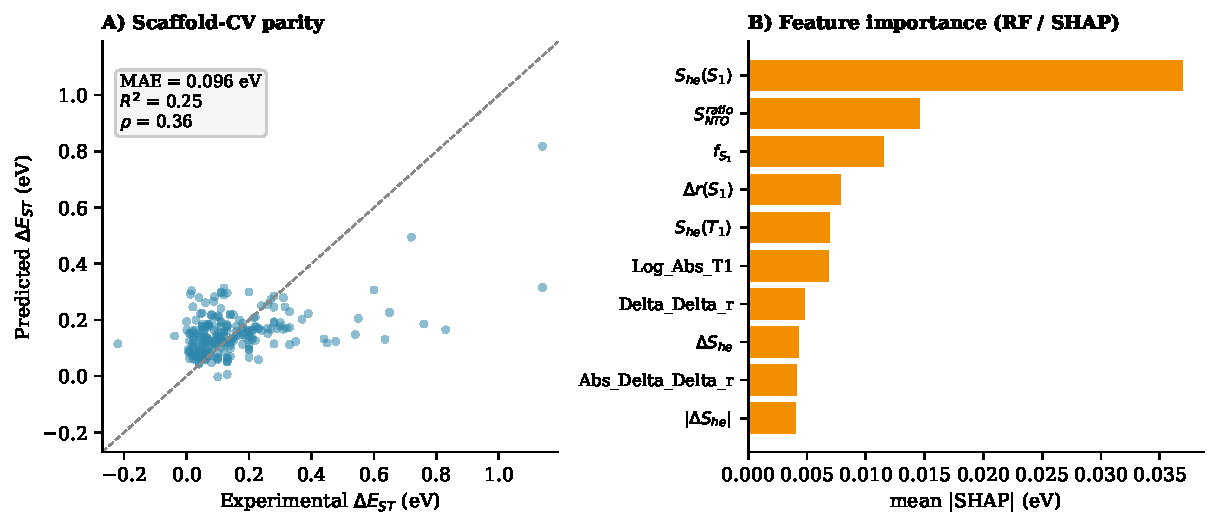
\includegraphics[width=0.95\textwidth]{figures/fig1_model_performance.pdf}
  \caption{Structure-based prediction of experimental $\Delta E_\text{ST}$.
    (A)~Scaffold cross-validated parity for the random forest on NTO
    spatial descriptors (\num{231} molecules, \num{212} Bemis--Murcko scaffolds):
    MAE = \qty{0.096}{\electronvolt}, $R^2 = 0.25$, Spearman $\rho = 0.36$. Models
    built from 2D structure alone (Morgan, RDKit) have similar errors
    (\cref{tab:feature_comparison}); formal equivalence was not established. The
    model regresses high-gap outliers toward the mean, the expected behaviour
    when the training distribution is dominated by low-gap emitters.
    (B)~SHAP importances: hole--electron overlap $S_\text{he}$, NTO overlap ratio,
    oscillator strength $f_{S_1}$ and charge-transfer distance $\Delta r$ dominate,
    consistent with exchange-integral physics.}
  \label{fig:model_performance}
\end{figure*}

We assembled \num{231} donor--acceptor molecules for which an experimental
$\Delta E_\text{ST}$ could be matched to a structure, and evaluated random-forest
regressors under Bemis--Murcko scaffold cross-validation (\num{212} distinct
scaffolds), so that no scaffold appears in both training and test.
Because \qty{92.9}{\percent} of scaffolds are singletons, scaffold and random splits
produce numerically similar folds (test--train nearest-neighbour Tanimoto differs by
only \num{0.022}). The scaffold split guarantees zero shared scaffolds per fold
(versus \numrange{3}{8} under a random split) but task difficulty barely changes;
the harder test of transfer is the source-paper split reported below.
That the model learns real signal rather than
scaffold-group structure is confirmed by a label-permutation test: the true
scaffold-CV MAE (\qty{0.096}{\electronvolt}) lies far below the null from
\num{1000} target shuffles (mean \qty{0.121}{\electronvolt}, $p = 0.001$;
Table~\ref{SI-tab:scaffold}).
The headline accuracy is also stable across validation schemes: replacing the singleton
scaffolds with genuine multi-molecule Butina clusters (down to \num{70} groups, largest
\num{38} molecules) leaves the MAE at \qtyrange{0.099}{0.104}{\electronvolt}, between
scaffold-CV (\qty{0.096}{\electronvolt}) and random-CV (\qty{0.106}{\electronvolt})
while preserving the rank correlation (Spearman $\rho$ spanning \numrange{0.31}{0.40} across cutoffs), showing that the ranking capability does not degrade under aggressive clustering
(Table~\ref{SI-tab:clustercv}).
The three feature sets perform within \qty{0.009}{\electronvolt} of one another
(\cref{tab:feature_comparison}); for the fingerprint and excited-state models, which we
compare head to head below, that closeness is backed by a paired bound of
\qty{0.017}{\electronvolt}. Two are computed from the 2D structure alone, with
no quantum chemistry: Morgan fingerprints (MAE = \qty{0.091}{\electronvolt}) and
RDKit physicochemical descriptors (\qty{0.100}{\electronvolt}). The third, NTO spatial
descriptors, is derived from a semi-empirical sTDA excited-state calculation but
excludes the $S_1$/$T_1$ energy scalars; it reaches MAE = \qty{0.096}{\electronvolt}
(\qty{95}{\percent} CI \numrange{0.082}{0.109}), $R^2 = 0.25$ (CI
\numrange{0.03}{0.45}), Spearman $\rho = 0.36$.
That the tested structure-only sets have similar errors to the NTO set is the
central comparison: the semi-empirical calculation has no measured error
advantage on these folds. Adding back the $S_1$/$T_1$ energies does not improve
the forest's MAE either (\cref{tab:feature_comparison}). The \emph{Energies~+~NTO}
set has MAE \qty{0.097}{\electronvolt} versus
\qty{0.096}{\electronvolt} for NTO alone. Similar predictive errors do not
establish that the feature sets encode identical physical information.
The natural comparator is the mean-value baseline (MAE = \qty{0.107}{\electronvolt}),
over which every model improves by only about \qty{10}{\percent}; the large apparent
gain over the raw sTDA gap (\qty{0.25}{\electronvolt}) reflects that the semi-empirical
gap is badly biased, not that the model is accurate.
The $R^2$ confidence intervals are wide and, for the structure-only sets, include
negative values (RDKit \numrange{-0.11}{0.51}; Morgan \numrange{-0.19}{0.53}): at
\qty{95}{\percent} confidence we cannot exclude that these models are no better than
predicting the mean. The signal is real but weak.

A higher level of theory does not change this picture. A range-separated TD-DFT
gap (wB97X-D4/def2-SVP, Tamm--Dancoff, \num{609} core-hours) overestimates the
measured gap by a systematic \qty{0.65}{\electronvolt} and, used directly, is the
least accurate predictor in \cref{tab:feature_comparison} (MAE
\qty{0.654}{\electronvolt}, $R^2 = -16.3$). Its correlation with experiment is
higher than the semi-empirical gap's (Pearson $r$ from \num{0.32} to \num{0.43}),
and an in-fold linear calibration that removes the offset brings it to MAE
\qty{0.099}{\electronvolt}---level with the mean-value baseline, still short of
the structure-only forest. Added as a single feature it lowers the Morgan model
from \num{0.091} to \qty{0.087}{\electronvolt} (paired \qty{95}{\percent} CI
\numrange{0.0004}{0.0071}, Wilcoxon $p = 0.016$): a small gain for
\num{609} core-hours (Table~\ref{SI-tab:tddft_headtohead}). This higher-level
TD-DFT descriptor is distinct from the semi-empirical NTO spatial set: the
latter does not lower the scaffold-CV error, whereas the former yields a
measurable but modest improvement.

Holding out whole source papers rather than scaffolds tests a different axis:
it removes entire publications and correlated chemical series. Because the corpus
records no measurement conditions per value, this is a proxy for shared practices,
not a laboratory- or protocol-controlled experiment. Under DOI-grouped five-fold
\texttt{GroupKFold} (\num{173} papers, \num{231} molecules) the Morgan model reaches
MAE \qty{0.102}{\electronvolt} ($R^2 = 0.18$; NTO $R^2 = 0.142$), and its paired advantage over the
mean-value baseline falls to \qty{0.005}{\electronvolt} with a \qty{95}{\percent}
CI that crosses zero. On accuracy, the model's advantage is not resolved under
this source-paper split.

Ranking behaves differently in these same folds: on this fixed fold assignment the NTO model has Spearman
$\rho = \num{0.35}$ while Morgan has \num{0.16} (MAE
\qty{0.099}{\electronvolt} against \qty{0.102}{\electronvolt}). Their paired
$\Delta\rho = \num{0.19}$ (the fixed-split value; the median over \num{50} random fold assignments is \num{0.16}, \cref{subsec:holdout_unit}) has a molecule-resampled \qty{95}{\percent} CI of
\numrange{0.04}{0.34}. Resampling the \num{173} primary source DOIs instead
gives \numrange{0.014}{0.366}; that paper-cluster interval barely excludes zero
and remains conditional on these fitted out-of-fold predictions. In \num{20}
additional paper-group partitions, retraining both models with \qty{20}{\percent}
of DOI groups held out each time, NTO has the higher test-set rank correlation
in \num{19} (median $\Delta\rho = \num{0.134}$; range
\numrange{-0.014}{0.404}). Those overlapping same-corpus partitions show
sensitivity to grouping rather than independent replication. Together these
tests identify a possible NTO ranking use case, not an advantage established
for selection in a new laboratory. One observation bounds the pessimistic reading, with a caveat that must travel with it:
\qty{58}{\percent} of repeatedly-measured molecules have zero inter-report spread, and
on the \num{102}-molecule multi-report subset the model reaches the study's lowest MAE,
\qty{0.080}{\electronvolt}. That subset is also an easier target: a mean-value predictor
restricted to it scores \qty{0.089}{\electronvolt}, so the model's advantage there is
\qty{0.009}{\electronvolt} with a \qty{95}{\percent} CI spanning zero. The low absolute
error reflects the narrower spread of those labels more than any gain in prediction.

\begin{table*}[t]
  \centering
  \caption{Prediction of experimental $\Delta E_\text{ST}$ under scaffold
    cross-validation (random forest, \num{231} molecules); $R^2$ with \qty{95}{\percent}
    bootstrap CI. The 2D-structure-only sets (no quantum chemistry) match the
    NTO set, which requires an sTDA excited-state run; none approaches the
    precision a quantitative photophysical method would require, and the
    structure-only $R^2$ intervals include zero. The range-separated TD-DFT
    reference gap (wB97X-D4/def2-SVP, Tamm--Dancoff; \num{609} core-hours) is
    listed raw, after an in-fold linear calibration, and as an added feature
    (Table~\ref{SI-tab:tddft_headtohead}).}
  \label{tab:feature_comparison}
  \begin{tabular}{lccc}
    \toprule
    Feature set & MAE (eV) & $R^2$ (\qty{95}{\percent} CI) & Spearman $\rho$ \\
    \midrule
    Morgan FP (2D structure only)   & 0.091 & 0.27 ($-0.19$, 0.53) & 0.31 \\
    RDKit desc.\ (2D structure only) & 0.100 & 0.31 ($-0.11$, 0.51) & 0.26 \\
    NTO spatial (needs sTDA)        & 0.096 & 0.25 (0.03, 0.45) & 0.36 \\
    Energies + NTO (reference)      & 0.097 & 0.24 & 0.34 \\
    \midrule
    Mean-value baseline             & 0.107 & 0.00 & --- \\
    Raw sTDA gap                    & 0.251 & $-2.22$ & 0.24 \\
    \midrule
    \multicolumn{4}{l}{\emph{Physics reference gaps (higher level of theory)}} \\
    Raw TD-DFT gap (wB97X-D4/def2-SVP) & 0.654 & $-16.3$ & 0.38 \\
    Calibrated TD-DFT gap (in-fold)    & 0.099 & 0.17 & 0.37 \\
    Morgan FP $+$ TD-DFT gap           & 0.087 & 0.31 & 0.37 \\
    \bottomrule
  \end{tabular}
\end{table*}

For the NTO variant, SHAP (SHapley Additive exPlanations) analysis
(\cref{fig:model_performance}B) identifies
hole--electron overlap $S_\text{he}$ (which governs the magnitude of the exchange interaction), the NTO overlap ratio (tracking transition purity), oscillator strength
$f_{S_1}$ (a proxy for transition dipole coupling), and the charge-transfer distance $\Delta r$ (which dictates spatial separation) as the dominant
predictors---physical quantities that jointly constrain the exchange integral governing
$\Delta E_\text{ST}$. This ranking is stable rather than an artefact of one fit:
across \num{200} bootstrap refits the leading descriptor $S_\text{he}(S_1)$ stays
in the top five \qty{99.5}{\percent} of the time, and on average \num{3.7} of the
five canonical descriptors recur (Table~\ref{SI-tab:shapboot}). Restricting the attribution to
the reliable-prediction subset---the \num{152} molecules whose out-of-fold residual is
below \qty{0.10}{\electronvolt}---leaves $S_\text{he}(S_1)$ ranked first in
\qty{99.5}{\percent} of refits, so the leading attribution does not rest on the
poorly-predicted tail. An independent, model-agnostic permutation-importance analysis ranks the same
descriptor, $S_\text{he}(S_1)$, first, so the leading attribution is corroborated by
two methods (the lower-ranked tail is not; SI section~S6.3). Given the model's modest
ranking power, we read only the dominant attribution as a mechanistic hypothesis for
experimental test rather than a validated causal claim; the structure-only
fingerprint and descriptor models reach the same accuracy without any excited-state
calculation.

\subsection{NTO and fingerprint models have similar error under scaffold holdout}\label{subsec:nto_null}

Do quantum-mechanical features beat pure structural descriptors when the target is an
experimental property? In scaffold cross-validation the tested NTO representation
does not reduce error. Paired on identical folds, the NTO model (MAE
$= \qty{0.096}{\electronvolt}$) and the Morgan model
($\qty{0.091}{\electronvolt}$) differ by
$\Delta\text{MAE} = \qty{-0.0043}{\electronvolt}$ for Morgan minus NTO
(\qty{95}{\percent} CI \numrange{-0.0171}{+0.0092}, Wilcoxon $p = 0.66$).
The lower confidence limit is close to the proposed
\qty{0.017}{\electronvolt} equivalence margin; we report the observed
similarity rather than claim a formal equivalence test. Both outperform the
mean-value baseline in paired comparisons, but neither predicts individual
gaps with the precision needed for emitter selection.

The accuracy comparison does not settle ranking on source-paper holdouts. In the
DOI-grouped folds (\cref{subsec:benchmark}), NTO retains Spearman
$\rho = 0.35$ while Morgan has $\rho = 0.16$; their paired difference on this fixed
fold assignment is $\Delta\rho = 0.19$ (paper-cluster \qty{95}{\percent} interval
\numrange{0.014}{0.366}), and the median over \num{50} fold assignments is
\num{0.16} (\cref{subsec:holdout_unit}). In a separate scaffold-CV triage analysis, at the
top \qty{20}{\percent} of the labelled benchmark NTO enrichment is
\num{1.6}-fold versus \num{1.4}-fold for Morgan.
The next subsection tests whether this ranking contrast comes from the evaluation
criterion or from the holdout unit. It does not establish that the contrast persists on
independent corpora or controlled protocols.
Recent theoretical work by Salvi et al.~\cite{Salvi2025} on electronic correlation
suggests a possible limitation of semi-empirical descriptors; the present
comparison alone cannot identify its cause.
The two representations differ in what they can be read for, though not in a way the
attribution totals establish on their own. The ten highest-attribution NTO descriptors
carry \qty{79}{\percent} of that model's SHAP weight against \qty{30}{\percent} for the
ten highest-attribution Morgan bits (Figure~\ref{SI-fig:shapcompare}); those totals are not
comparable, because ten descriptors are \qty{29}{\percent} of the \num{35}-dimensional
NTO set and ten bits are \qty{0.5}{\percent} of a \num{2048}-bit fingerprint, so the
concentration follows from dimensionality. What does not follow from dimensionality is
that the NTO features are \emph{named} donor--acceptor overlap and charge-transfer
quantities, whereas Morgan bits are anonymous hashed substructures. The case for the
physics-informed representation is interpretability of the variables themselves, not a
larger share of attribution.

\subsection{Fingerprint ranking depends on same-publication molecules}\label{subsec:holdout_unit}

The holdout unit, not the error-versus-ranking criterion, sets the size of the NTO--Morgan rank
contrast. We repeated the comparison with \num{50} random assignments of groups to five folds for
each of three units (\cref{tab:holdout_unit}). Under source-paper holdout the median
$\Delta\rho$ (NTO minus Morgan) is \num{0.160} and is positive in \num{50} of \num{50} assignments;
under scaffold holdout it is \num{0.073} (\num{49}/\num{50} positive) and under random
molecule holdout \num{0.055} (\num{45}/\num{50} positive). The \num{0.191} of the fixed
split lies in the upper part of the paper-holdout distribution, so the fold-assignment-robust
value is $\approx\num{0.16}$ (\num{50}-assignment range \numrange{0.07}{0.25}); the ranges
describe fold-assignment variability, not confidence intervals. The error comparison does not move
with the unit: Morgan minus NTO MAE is \qty{-0.0004}{\electronvolt} under paper holdout and
\qty{-0.0045}{\electronvolt} under scaffold holdout, with ranges that span zero, and
\qty{-0.0081}{\electronvolt} under random holdout, where Morgan is slightly better
(range \numrange{-0.0157}{-0.0002}). NTO is higher in \num{19} of \num{20} repeated
paper-group partitions, against \num{11} of \num{20} for scaffold and \num{13} of \num{20}
for molecule partitions, so the earlier \num{19}/\num{20} count is specific to the paper unit.

\begin{table}[htbp]
  \centering
  \caption{Rank correlation of random-forest models by holdout unit (same \num{231}
    molecules; \num{50} random group-to-fold assignments, medians). $\Delta\rho$ is NTO minus Morgan;
    the range is the 2.5th to 97.5th percentile over assignments, a measure of
    fold-assignment variability, not a confidence interval. The last column counts
    \num{20} repeated holdout partitions in which NTO has the higher test-set $\rho$.
    RDKit 2D descriptors were run under molecule and paper holdout only (n.t., not tested);
    their multi-paper $\rho$ falls from \num{0.518} to \num{0.350} and single-paper $\rho$ under
    paper holdout is \num{0.102}.}
  \label{tab:holdout_unit}
  \footnotesize\setlength{\tabcolsep}{1.5pt}
  \begin{tabular}{lcccccc}
    \toprule
    & & & \multicolumn{3}{c}{median $\rho$} & NTO \\
    \cmidrule(lr){4-6}
    Unit (groups) & $\Delta\rho$ & Range & Morgan & RDKit & NTO & higher \\
    \midrule
    Paper (\num{173})    & 0.160 & 0.073--0.246 & 0.172 & 0.209 & 0.337 & 19/20 \\
    Scaffold (\num{212}) & 0.073 & 0.007--0.144 & 0.269 & n.t. & 0.351 & 11/20 \\
    Molecule (\num{231}) & 0.055 & $-0.033$--0.126 & 0.305 & 0.303 & 0.352 & 13/20 \\
    \bottomrule
  \end{tabular}
\end{table}

The contrast comes from the fingerprint side. NTO rank correlation is nearly invariant to the unit
(median $\rho$ \numrange{0.337}{0.352}), whereas Morgan $\rho$ falls from \num{0.305} (random) to
\num{0.269} (scaffold) to \num{0.172} (source paper) (\cref{fig:holdout_unit}a). Splitting the
molecules by paper multiplicity locates the drop (\cref{fig:holdout_unit}b). For the \num{103}
molecules whose paper contributes at least one other molecule, Morgan $\rho$ is \num{0.54} when
siblings are in training and \num{0.26} when the whole paper is held out, while NTO moves from
\num{0.48} to \num{0.45}. For the \num{128} molecules from single-molecule papers, Morgan $\rho$ is
\num{0.10} under either holdout against \num{0.24} for NTO; with predictions averaged over the
\num{50} paper-holdout assignments the two are \num{0.11} and \num{0.27}, a difference of
\num{0.16} whose paired bootstrap \qty{95}{\percent} CI (\numrange{-0.05}{0.37}) includes zero,
so this subset contrast is not resolved. The sibling-pull statistic, the Spearman
correlation between a molecule's prediction and the mean label of its same-paper siblings, is
\num{0.68} for Morgan under random holdout and \num{0.26} under paper holdout, against \num{0.47} and
\num{0.42} for NTO. Morgan's MAE on multi-paper molecules is \qty{0.025}{\electronvolt} lower under random
than under paper holdout (range \numrange{0.014}{0.034}); NTO's difference is
\qty{0.007}{\electronvolt}, with a range that includes zero.

A dense descriptor set without quantum chemistry behaves like the fingerprint. The \num{217}
RDKit 2D descriptors, run through the same \num{50} assignments, reach median $\rho$ \num{0.303}
under random and \num{0.209} under paper holdout; on multi-paper molecules $\rho$ falls from
\num{0.518} to \num{0.350}, and on single-paper molecules it is \num{0.102}
(\cref{tab:holdout_unit}). Among the three sets tested, holdout-unit invariance is specific to
the NTO descriptors, and dimensionality alone does not explain it. None of the three orders
molecules \emph{within} a held-out paper: the Spearman correlation between paper-centred labels and
paper-centred predictions on the \num{103} multi-paper molecules is \num{-0.06} to \num{0.03}
under paper holdout. The NTO advantage is in ordering emitters across publications absent from
training. Under random holdout Morgan's within-paper $\rho$ is \num{-0.35}: its predictions are
pulled towards the sibling mean, which inverts the order inside a paper.

\begin{figure}[t]
  \centering
  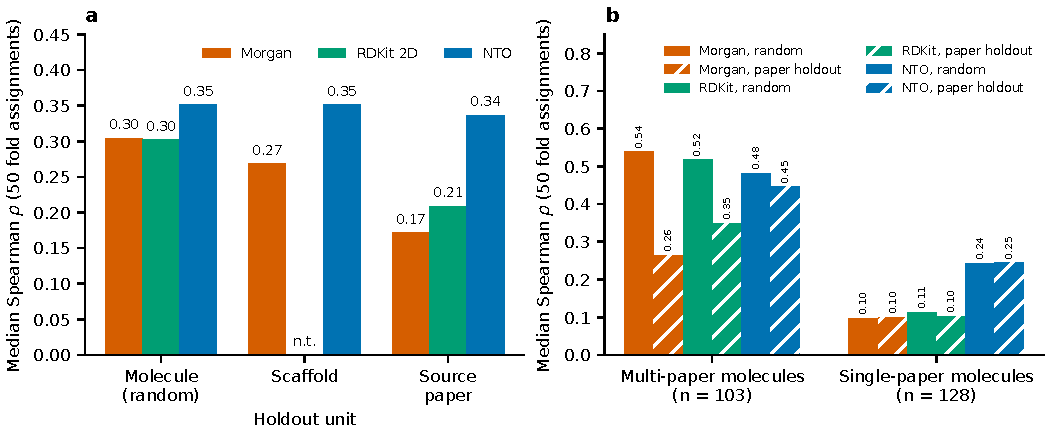
\includegraphics[width=\columnwidth]{figures/holdout_unit_ranking.pdf}
  \caption{Rank correlation by holdout unit and by paper multiplicity (medians over \num{50} random
    fold assignments; random-forest models on the same \num{231} molecules). (a)~Spearman $\rho$ for
    Morgan, RDKit 2D and NTO features under molecule, scaffold and source-paper holdout (RDKit was
    not run under scaffold holdout; n.t.). (b)~$\rho$ for the \num{103} molecules from
    multi-molecule papers and the \num{128} from single-molecule papers, under random and paper
    holdout. The full seed-range tables are in the SI.}
  \label{fig:holdout_unit}
\end{figure}

This is an association. Molecules from one paper share close structure and measurement protocol,
and these tests cannot separate structural near-duplication from laboratory or protocol effects. The
paper-multiplicity test compared random with source-paper holdout only (scaffold holdout was not
part of it): the fingerprint model's ranking skill under random holdout sits mostly on molecules whose
same-paper siblings are in training, and the NTO descriptors keep their rank information when
the siblings are absent. All units use one corpus and \num{128} of the \num{173} papers contribute a
single molecule, so paper holdout differs from random holdout through the \num{45} multi-molecule papers
only; no test here crosses laboratories.

\subsection{Label scatter leaves the ceiling at $R^2_\text{max} \approx 0.8$, well above the observed $R^2$}\label{subsec:ceilings}

The observed MAE is near \qty{0.1}{\electronvolt}, but label variability does
not by itself account for the model's error.
Independent experimental reports for the same compound disagree
substantially: a single randomly chosen report sits \qty{0.072}{\electronvolt} from its
molecule's median (RMS with each molecule weighted equally), the disagreement exceeds the
model MAE for \qty{19.6}{\percent} of molecules, and the worst molecule reaches a standard
deviation of \qty{0.56}{\electronvolt}; the eight independent values for 4CzIPN alone span
\qtyrange{0.01}{0.48}{\electronvolt} (Table~\ref{SI-tab:solvent}). This scatter is consistent with uncontrolled measurement conditions (solvent polarity, concentration, host matrix), which influence photophysical measurements~\cite{Dang2025}; the corpus cannot separate conditions, protocol and transcription error. That $\Delta E_\text{ST}$
is reported inconsistently has been shown for individual emitters~\cite{Shuaib2026};
quantified across \num{231} molecules and \num{173} source papers it provides
an inter-report variability estimate for this TADF corpus. This variability
constrains any predictor fitted to the measured labels.
The quantity the model is regressed on, however, is the per-molecule \emph{median}.
For the \num{102} molecules with several reports, the RMS standard error of that median
is \qty{0.049}{\electronvolt}; the other \num{129} labels rest on one report each, and
counting them at single-report scatter gives an RMS label noise of about
\qty{0.072}{\electronvolt} over all \num{231} molecules. Label imprecision is therefore
a real term in the error budget but does not by itself account for it, and we do not
claim the forest sits at a noise floor.
Applying the noise-ceiling framework of Crusius et al.~\cite{Crusius2025}
($R^2_\text{max} = 1 - \sigma^2_\text{noise}/\sigma^2_y$) with per-molecule noise
(the standard error of the mean for the \num{102} multi-report molecules, and the
single-report scatter for the \num{129} single-report molecules) gives
$R^2_\text{max} \approx 0.81$ (\qty{95}{\percent} CI \numrange{0.68}{0.88}) for the
pooled within-molecule SD of \qty{0.0856}{\electronvolt}; the alternative single-report
estimates give \num{0.80} and \num{0.86}. All lie well above the observed $R^2 \approx 0.26$.
The model captures about \qtyrange{30}{32}{\percent} of that ceiling, so label noise alone is not the dominant
constraint. The assumptions behind the ceiling are listed in SI section~S3.3b.
Progress requires both a better dataset \emph{and} improvements in features or
corpus scale; label noise (about \qty{0.072}{\electronvolt} RMS over the \num{231}
molecules) is the term a curated benchmark would directly attack.
A second, separate dispersion applies to computed references rather than to this
regression: the computed gap is functional-dependent. Across the
\num{7} molecules (gas and toluene) for which we ran both B3LYP/6-31G(d) and CAM-B3LYP/def2-TZVP,
$\Delta E_\text{ST}$ differs by a mean \qty{0.30}{\electronvolt} (up to
\qty{0.58}{\electronvolt}) and changes
relative magnitude (Table~\ref{SI-tab:dft_benchmark}); a higher-tier benchmark across
six range-separated functionals on \num{27} emitters~\cite{Froitzheim2024} shows the same
effect at finer resolution: a median inter-functional spread of \qty{0.05}{\electronvolt}
on a quantity that approximates \emph{half} the gap, hence roughly
\qty{0.1}{\electronvolt} on \deltaest\ itself. Any claim of sub-\qty{0.1}{\electronvolt}
accuracy against such a reference is not physically meaningful. This second effect bounds
what a \emph{computed} gap can mean; it does not bound a model regressed on measured
labels, and we do not add the two into a single floor. Only the label term applies
directly to the present task. Among the representations tested here, larger
learner capacity does not close the gap. Histogram gradient boosting reaches
\qty{0.105}{\electronvolt}, an MLP \qty{0.169}{\electronvolt} and an RBF SVR
\qty{0.120}{\electronvolt} (Table~\ref{SI-tab:capacity}); a second comparison over a
differently configured set of learners places plain gradient boosting at
\qty{0.098}{\electronvolt}, within \qty{0.002}{\electronvolt} of the forest and well below the proposed
\qty{0.017}{\electronvolt} comparison margin
(Table~\ref{SI-tab:capacity} lists the
histogram-boosting configuration). A frozen pretrained SMILES transformer (ChemBERTa,
\num{77}M parameters), the representation a current screening pipeline would reach for
first, is no exception: its mean-pooled embeddings feed a random-forest or ridge head
to MAE \qtyrange{0.109}{0.113}{\electronvolt} on the same scaffold folds---it does not
beat the \qty{0.107}{\electronvolt} mean-value baseline, and is worse than Morgan by a
paired \qty{0.022}{\electronvolt} (\qty{95}{\percent} CI \numrange{0.008}{0.034},
excluding zero; \texttt{code/a013\_pretrained\_encoder\_baseline.py}). Fine-tuning this encoder on only \num{231} labels was not tested here.
Among the representations evaluated, added capacity did not improve the
measured-gap error; this does not exclude other architectures or training sets.
The negative lower $R^2$ bound is not a
fingerprint-width artefact, since \num{512}-, \num{1024}- and \num{2048}-bit Morgan models
share it (Table~\ref{SI-tab:capacity}).

Stratifying by label quality does not isolate a label effect. Restricting to molecules that carry replicates, the model reaches MAE
\qty{0.074}{\electronvolt} on the \num{79} whose reports agree to
$\le\qty{0.05}{\electronvolt}$, \qty{0.106}{\electronvolt} on the \num{23} whose
reports do not, and \qty{0.107}{\electronvolt} on the \num{129} for which label
precision cannot be measured. That ordering is not evidence about labels: a constant
predictor fitted within each stratum reproduces it almost exactly
(\qty{0.074}{}, \qty{0.107}{} and \qty{0.110}{\electronvolt}), because the strata
differ in the dispersion of the target itself (standard deviation \qty{0.10}{},
\qty{0.15}{} and \qty{0.20}{\electronvolt}). Within any one stratum the model carries
no advantage over a constant. We therefore report no stratified evidence for a label
ceiling; the quantitative statement that survives is the label-noise estimate above.

A related question is whether \emph{uncontrolled measurement conditions}, rather than
label imprecision as such, set the limit. The corpus records no solvent, host or
temperature for individual values, so a strictly condition-controlled subset cannot be
built; the closest available grouping is by source paper, without a guarantee that
measurements in one publication share a laboratory or solvent. Splitting the benchmark on that
(\num{218} single-source against \num{13} multi-source molecules) and scoring the random
forest on scaffold cross-validation folds, the model's descriptive advantage
over a constant fitted within each full group is \qty{0.0071}{} and
\qty{0.0024}{\electronvolt}, respectively. The latter comparator is not held out:
a separate out-of-fold recalculation gives \qty{0.1006}{\electronvolt} and
\qty{0.0693}{\electronvolt} for the single- and multi-source groups. The old
group-difference interval (\numrange{-0.014}{0.035}) used the in-sample constants
and must not be interpreted as a matched predictive comparison. The raw
errors run the other way (\qty{0.058}{} against \qty{0.093}{\electronvolt}) but the
multi-source group's target dispersion is half as large and its in-sample constant
scores \qty{0.061}{\electronvolt}; the held-out constant scores
\qty{0.069}{\electronvolt} instead. With only \num{13} molecules drawing on
more than one source paper, neither a benefit nor a penalty of mixed source
membership is resolved by these comparisons. The corpus does not permit a
controlled test of solvent or measurement protocol.

A larger but differently processed corpus gives a stress test, not an isolated
sample-size experiment. Featurising \num{497} additional
experimental emitters through the same pipeline (a \num{728}-molecule set) raises
the MAE from \qty{0.098}{} to \qty{0.124}{\electronvolt}, drives $R^2$ from
\num{0.18} to $-0.01$, and roughly halves the rank correlation (Spearman $\rho$
from \num{0.34} to \num{0.16}); the replicate-measured subset
($n = \num{465}$) recovers only about half of the loss (Table~\ref{SI-tab:expansion}).
In this expanded, differently processed set, prediction worsens rather than
improves. The added molecules were resolved through a different structure
pipeline, so broader chemistry, target quality, and preprocessing are confounded;
the comparison cannot determine whether corpus size alone helps or hurts.

A separate concern is the descriptor side: the NTO features are computed at the
\emph{vertical} (ground-state) geometry, whereas the measured gap reflects relaxed
excited states. We bounded this approximation by recomputing \deltaest\ adiabatically
for \num{14} representative emitters in gas and toluene at CAM-B3LYP/def2-TZVP with
excited-state optimisation (Table~\ref{SI-tab:adiabatic}). Relative to these adiabatic
references the vertical gap carries a mean absolute deviation of
\qty{0.195}{\electronvolt}, which exceeds the model's own error. The deviation is
dominated by an additive offset rather than by reordering---a linear fit gives slope
\num{1.00} and intercept \qty{0.07}{\electronvolt} ($R^2 = 0.70$, Spearman
$\rho = 0.71$)---so relaxation shifts the scale more than it scrambles the ranking the
triage relies on. The residual is not negligible, however: the RMS deviation is
\qty{0.245}{\electronvolt} and the worst molecule departs by \qty{0.548}{\electronvolt},
with sign changes between compounds, and \num{14} molecules cannot settle how much of
that is systematic. We take the vertical descriptors as an acceptable ranking input on
this evidence, not as a validated approximation to the adiabatic gap.

Candidate triage (enrichment \num{1.2}--\num{1.4}$\times$ over random for low-gap emitters,
established only at cutoffs of about \num{50} molecules or a fifth of the benchmark) and the
\num{22194}-structure substructure-filtered library, where split-conformal intervals rule out
single-molecule selection, are reported in SI section~S6.7.

\subsection{The cited TADF-gap models report error on computed gaps, not ranking across held-out publications}\label{subsec:comparison}

The low errors reported for TADF-gap models are obtained against computed targets:
a TD-DFT gap inside a $>$\num{1000000}-molecule screen~\cite{Gomez-Bombarelli2016},
semi-empirical gaps over a virtual library~\cite{Thapa2025}, ADC(2) gaps of
inverted-gap molecules reproduced to \qty{0.02}{\electronvolt}~\cite{Barneschi2024},
quasiparticle-corrected Kohn--Sham gaps for \num{233} INVEST and TADF molecules at
\qty{0.06}{\electronvolt}~\cite{Li2026}, and $\omega$B2PLYP$'$ gaps that Nigam
et al.\ moved from regression to a good/bad classifier~\cite{Nigam2024}
(Table~\ref{SI-tab:prior_ml}). He et al.~\cite{He2026} trained on \num{1321}
measured gap records with measurement-condition features but did not compare
fingerprint and semi-empirical NTO representations under molecule, scaffold and
source-publication holdout.
Against measured gaps, whose labels carry about \qty{0.072}{\electronvolt} RMS of
inter-report noise, the Morgan and NTO models reach \qtyrange{0.091}{0.096}{\electronvolt},
\qtyrange{10}{15}{\percent} below the mean-value predictor (naive baselines in
Table~\ref{SI-tab:baselines}). Whether the computed-gap estimators keep their
accuracy against measured gaps has not been tested, and none of these studies reports how ranking holds when whole publications are held out, the test made in \cref{subsec:holdout_unit}.

\subsection{Limitations}\label{subsec:limitations}

All results come from one corpus of \num{231} molecules, so the holdout-unit comparison does not
test transfer to a new laboratory or a controlled protocol. The target is a consensus
literature value (inter-report RMS scatter \qty{0.072}{\electronvolt}) of a single scalar,
$\Delta E_\text{ST}$; solvatochromic, conformer-dependent and device-level quantities are not
predicted. The NTO descriptors use ground-state vertical geometries (mean absolute deviation
\qty{0.195}{\electronvolt} from adiabatic references for \num{14} emitters), inverted-gap
emitters are out of scope (both negative labels receive positive predictions), and only
tabular learners and one frozen pretrained encoder were tested. Ranking is moderate
($\rho \approx 0.34$ to $0.36$), so the models support triage, not selection. The full list is in
SI section~S6.8.

% ============================================================
% JMGM Conclusions — F3-b re-scope (2026-10-06); no numbers beyond Results.
% ============================================================

\section{Conclusions}\label{sec:conclusions}

Do semi-empirical NTO descriptors retain rank information on measured TADF
singlet--triplet gaps that structural fingerprints lose when molecules come from
publications absent from training? In this corpus they do: under source-paper
holdout the NTO model orders emitters across publications absent from training with
median Spearman $\rho = 0.34$, against $0.17$ for Morgan fingerprints. The
contribution is a matched three-unit holdout comparison showing that fingerprint
and RDKit ranking of measured TADF gaps depends on same-publication molecules in
training, while semi-empirical NTO ranking does not. Neither representation orders
molecules within a held-out paper, and neither has lower error than the other.
Three results delimit that answer.

\paragraph{Fingerprint and NTO models do not differ in error.}
Random forests built from the 2D structure alone---Morgan fingerprints
(MAE = \qty{0.091}{\electronvolt}) and RDKit descriptors
(\qty{0.100}{\electronvolt})---predict experimental $\Delta E_\text{ST}$ as well
as NTO descriptors derived from a semi-empirical excited-state calculation
(\qty{0.096}{\electronvolt}), against \qty{0.107}{\electronvolt} for the mean-value
predictor; the paired Morgan-minus-NTO MAE difference has a \qty{95}{\percent} CI of
\numrange{-0.0171}{+0.0092}~eV, and it stays near zero under paper holdout. Both
the Morgan and NTO models sit only \qtyrange{10}{15}{\percent} below the mean. This
null settles one design question: the sTDA calculation is not justified by
accuracy, and its measurable value is ranking across publications. The
\qtyrange{10}{15}{\percent} margin over the mean is the bar a new structure
representation has to clear on these labels.

\paragraph{The holdout unit, not the metric, sets the ranking contrast.}
The NTO-minus-Morgan $\Delta\rho$ is \num{0.16}
under source-paper holdout (\qtyrange{2.5}{97.5}{\percent} span \numrange{0.07}{0.25} over \num{50} fold
assignments) against \num{0.073} under scaffold and \num{0.055} under molecule
holdout. NTO ranks higher in \num{19} of \num{20} repeated paper partitions, but in
only \num{11} and \num{13} of \num{20} matched scaffold and molecule partitions, so
the \num{19}/\num{20} count belongs to the paper unit. The contrast comes from the
fingerprint side: NTO $\rho$ is nearly constant across units, while Morgan $\rho$
falls from \num{0.305} to \num{0.172}, and RDKit 2D descriptors fall with it
(\num{0.303} to \num{0.209}), so among the three sets tested the invariance is
specific to the NTO descriptors. Morgan ranks mainly molecules whose same-paper
siblings are in training; on molecules from single-molecule papers its $\rho$ is
\num{0.10}, and the NTO-minus-Morgan contrast on those molecules is not resolved
(\qty{95}{\percent} CI \numrange{-0.05}{0.37}). Siblings share both close structure
and measurement protocol, so this is an association, not an identified cause. SHAP
on the NTO variant ties the learned signal to hole--electron overlap and
charge-transfer character; it is an interpretable association, not a causal
validation.

Independent reports of the same compound
scatter by \qty{0.072}{\electronvolt} RMS. For the \num{102} multi-report molecules
the median label has an RMS standard error of \qty{0.049}{\electronvolt}; over all
\num{231} labels the estimated noise is about \qty{0.072}{\electronvolt} RMS, a
measurable part of the error budget but not all of it. Across \num{231}
molecules and \num{173} source papers, the report scatter supplies a direct
estimate of measurement variability. Error is lower on molecules whose
replicate reports agree (\qty{0.074}{\electronvolt} against
\qty{0.106}{\electronvolt}), but a constant predictor reproduces that ordering:
it reflects different spreads of the target, not evidence that removing label
noise alone improves the model. The estimated ceiling,
$R^2_\text{max} \approx 0.80$--\num{0.86}, lies well above the observed
$R^2 \approx 0.26$. In the tested representation set a frozen
pretrained molecular-transformer embedding reaches MAE
\qtyrange{0.109}{0.113}{\electronvolt}, worse than the Morgan model; other
representations remain untested. Separately, the computed gap is functional-dependent (mean
\qty{0.30}{\electronvolt}, up to \qty{0.58}{\electronvolt} between B3LYP and
CAM-B3LYP); this concerns computed references, not the experimental-label
noise estimate.

For modellers the consequence is practical. On literature-mined data, random and
scaffold splits leave same-paper siblings in training and, in this corpus, overstate
fingerprint ranking skill; a source-publication holdout should be reported with them
before a representation is chosen for ranking. Where ranking on unseen publications
matters, the semi-empirical NTO calculation is the representation that kept its rank
information here: it orders emitters across publications absent from training,
although no representation orders molecules within a held-out paper. As a triage filter the structure-based model enriches low-gap
candidates \numrange{1.2}{1.4}$\times$ over random selection at broad cutoffs; at
top-10 or top-20 the confidence intervals include random selection, and on the
filtered library the conformal intervals are too wide for molecule-level selection,
so no ranked shortlist is deposited.

All results come from one corpus of \num{231} molecules: the holdout-unit comparison
does not test transfer to a new laboratory or a controlled protocol, and
\num{128} of the \num{173} papers contribute a single molecule. The target is one
scalar, $\Delta E_\text{ST}$; the vertical NTO descriptors depart from adiabatic
references by \qty{0.195}{\electronvolt} on average for \num{14} emitters, and the
data do not support molecule-specific spin--orbit-coupling, $k_\text{RISC}$,
emission-wavelength or external-quantum-efficiency estimates
(\cref{subsec:limitations}).

\paragraph{What a controlled benchmark could resolve.}
Label noise of about \qty{0.072}{\electronvolt} RMS over the \num{231} molecules motivates
single-source, solvent-controlled measurements, with documented host and
protocol. Such a benchmark would separate measurement scatter from the
remaining modelling headroom; it does not follow from these data that a
better model could not improve on the current result.


\section*{Funding}
This research received no specific grant from any funding agency in the public,
commercial, or not-for-profit sectors.
\section*{Declaration of competing interest}
The authors declare no competing interests.
\section*{Author contributions}
J.-P.T.N.: Conceptualization, Methodology, Software, Validation, Formal analysis, Investigation, Data curation, Writing -- original draft, Visualization.
S.C.T.K.: Software, Validation, Writing -- review \& editing.
P.S.M.K.: Validation, Writing -- review \& editing.
P.S.: Resources, Validation, Writing -- review \& editing.
S.G.N.E.: Supervision, Project administration, Writing -- review \& editing.
\section*{Data and code availability}
The measured \deltaest labels come from the ChemDataExtractor-generated TADF
database of Huang and Cole~\cite{HuangCole2024}. Data, code and the full analysis ledger for the three related articles are publicly archived
under the Zenodo concept DOI 10.5281/zenodo.17436069, which resolves to the latest
version, and are mirrored at
\url{https://github.com/TchapetNjafa/Data_Articles_TADF}.
The scripts and outputs of the source-paper holdout and holdout-unit analyses
(ledger entries A-016 to A-020) are in that archive (\texttt{ML\_reproducibility/code}
and \texttt{ML\_reproducibility/data}). They are also enclosed as Supplementary Data,
in the folder \texttt{supplementary\_data/} and the archive
\texttt{JMGM\_group\_ranking\_supplement.zip}. The files are, code: \texttt{jmgm\_doi\_group\_ranking\_check.py}, \texttt{\_dataset.py}, \texttt{a017\_split\_unit\_controls.py}, \texttt{a018\_noise\_ceiling\_heterogeneous.py}, \texttt{a019\_series\_shortcut\_test.py}, \texttt{a020\_controls.py}, \texttt{fig\_holdout\_unit\_ranking.py}; data: \texttt{a016\_jmgm\_doi\_group\_input.csv}, \texttt{a016\_jmgm\_doi\_group\_ranking.json}, \texttt{a017\_split\_unit\_controls.json}, \texttt{a018\_noise\_ceiling\_heterogeneous.json}, \texttt{a019\_series\_shortcut\_test.json}, \texttt{a020\_controls.json} and \texttt{a006\_equivalence\_ceiling.json}.
\section*{Declaration of generative AI and AI-assisted technologies in the manuscript preparation process}
In preparing this work the authors used AI assistants (Claude by Anthropic --- Sonnet
4.5, accessed May~2026; Sonnet~5 and Opus~5, accessed September~2026 --- and ChatGPT by
OpenAI) for literature triage, \LaTeX{} formatting and consistency checking,
drafting and revision of manuscript text, and analysis scripts used for paired
comparisons, enrichment, label-precision audits and model baselines. The current
revision (October~2026) used Claude Code (Opus~5.5 and Sonnet~5.5, Anthropic)
for the holdout-unit control scripts, drafting and consistency checking, and
OpenAI Codex (GPT-6) and GitLab Duo for independent review checks; every
number was verified against the deposited analysis outputs. The graphical
abstract was rendered by an AI image generator from an author-written
specification. No AI system is listed
as an author. The human authors retain responsibility for the final text,
methods, figures and interpretation.
% AUTHOR ACTION: verify all AI tool names/dates and approve this disclosure.
\section*{Acknowledgements}
The authors thank Prof. Gian-Marco Rignanese (UCLouvain) for scientific advice and
access to high-performance computing facilities.

\bibliographystyle{elsarticle-num}
\bibliography{references_jmgm}
\end{document}
